
\documentclass[11pt, titlepage, twoside]{article}
\usepackage[top=20mm, bottom=20mm, left=20mm, right=20mm]{geometry}
\geometry{a4paper}
\geometry{portrait}
\usepackage[utf8]{inputenc}	% Comment out for xelatex; must use with pdflatex
\usepackage[T1]{fontenc}
\usepackage[parfill]{parskip} % Activate to begin paragraphs with an empty line rather than an indent
\usepackage{graphicx}
\usepackage{amsmath}
\usepackage{amssymb}
%\usepackage{fontspec}
\usepackage{epstopdf}
\usepackage{float}
\usepackage[hang]{footmisc}
\usepackage{endnotes}
\usepackage{listingsutf8}
%\restylefloat{table}
\usepackage{xcolor}
\usepackage{colortbl}
%\usepackage{booktabs}
\usepackage{tabu}
\usepackage{caption}
\usepackage{textcomp}
\usepackage{textgreek}

\usepackage{subcaption}\usepackage[style=numeric,backend=bibtex8]{biblatex}
\addbibresource{references.bib}
\usepackage{longtable}
\usepackage{csvsimple}				% for reading cvs files into tables

\makeatletter
\def\blx@maxline{77}
\makeatother

\captionsetup[figure]{labelfont=sc}
\captionsetup[table]{labelfont=sc}
\captionsetup[tabu]{labelfont=sc}

\DeclareCaptionType{MPEquation}[][List of equations]
\captionsetup[MPEquation]{labelformat=empty}

\DeclareCaptionType{MPListing}[][List of listings]
\captionsetup[MPListing]{labelformat=empty}

\usepackage{fancyhdr}
\setlength{\headheight}{16pt}
\pagestyle{fancyplain}
\fancyhf{}
%\fancypagestyle{plain}{}
\cfoot[\thepage]{\thepage}

\usepackage{stringenc}
\usepackage{pdfescape}


% Helper for debugging pdflatex errors induced by invalid UTF8 characters:
% output the actual character code causing the issue.

\makeatletter
\renewcommand*{\UTFviii@defined}[1]{%
\ifx#1\relax
\begingroup
% Remove prefix "\u8:"
\def\x##1:{}%
% Extract Unicode char from command name
% (utf8.def does not support surrogates)
\edef\x{\expandafter\x\string#1}%
\StringEncodingConvert\x\x{utf8}{utf16be}% convert to UTF-16BE
% Hexadecimal representation
\EdefEscapeHex\x\x
% Enhanced error message
\PackageError{inputenc}{Unicode\space char\space \string#1\space
(U+\x)\MessageBreak
not\space set\space up\space
for\space use\space with\space LaTeX}\@eha
\endgroup
\else\expandafter
#1%
\fi
}
\makeatother

% Make multi-paragraph footnotes align nicely on the left
\setlength\footnotemargin{10pt}

% Do not display an automatic Notes heading for endnotes, as they are contained
% by a Manuscripts section with a heading that has possibly been edited by the user
\def\enoteheading{}

% Apply footnote and endnote numbering schemes (decimal, lowercase roman etc.)
\renewcommand{\thefootnote}{\arabic{footnote}}
\renewcommand{\theendnote}{\arabic{endnote}}
% Adjust endnotes to use normal-sized numbering and text
\renewcommand{\enotesize}{\normalsize}
\renewcommand\enoteformat{%
  \raggedright
  \leftskip=1.8em
  \makebox[0pt][r]{\theenmark. \rule{0pt}{\dimexpr\ht\strutbox+\baselineskip}}%
}

\renewcommand*{\thefootnote}{\fnsymbol{footnote}}

%add 'S' prefix to figure and section 
\renewcommand{\thefigure}{S\arabic{figure}}
\renewcommand{\thesection}{S\arabic{section}}

\begin{document}


\section{Supplemental}\label{sec:supp}

\subsection{High vs. Low Confidence EEG Clusters}
\label{sec:deevEEGConf}
Here trials were selected based on the confidence ratings given for each retrieval attempt with the intention of capturing differences in EEG time frequency for Recollection vs. Familiarity based memory retrieval.  The same analysis approach used in the closed-loop vs. open-loop results was adopted for this confidence contrast (i.e. cluster based search in Stimulus Locked and Response Locked within theta, alpha and beta frequency bands).  All correctly retrieved trials with confidence rating less then 3 were assigned to the Low Confidence condition, and all correctly retrieved trials with confidence greater then 2 were assigned to the High Confidence condition (trial counts: low confidence correct $\mu=25\pm4$ 95\% confidence interval across subjects, high confidence correct $\mu=127\pm33$).  It should be noted that this difference in trial counts per condition should not impact the type 1 error rate of the cluster statistics as significance is calculated through a bootstrapped random permutation of condition labels across subjects.

Figure \ref{fig:deevConfClusters} shows the only 3 clusters found using the $p<0.05$ criteria; all clusters were found in the Response Locked epochs.  The theta cluster showed a greater increase in power relative to baseline for the High Confidence condition compared to Low Confidence, had a temporal extent from -3000 ms to -680 ms Response Locked, and its $t$-value mass was centered in left posterior electrodes.  In contrast, the alpha cluster showed a greater decrease in power for the Low Confidence condition compared to High Confidence, had a temporal extent from -3000 ms  to -480 ms Response Locked, and its $t$-value mass was in central posterior electrodes.  Similarly the beta cluster showed a greater decrease in power for the Low Confidence condition compared to High Confidence, had a temporal extent from -3000 ms to -1600 ms Response Locked, and its $t$-value mass was centered in right anterior electrodes.


\begin{figure}
	\begin{center}
		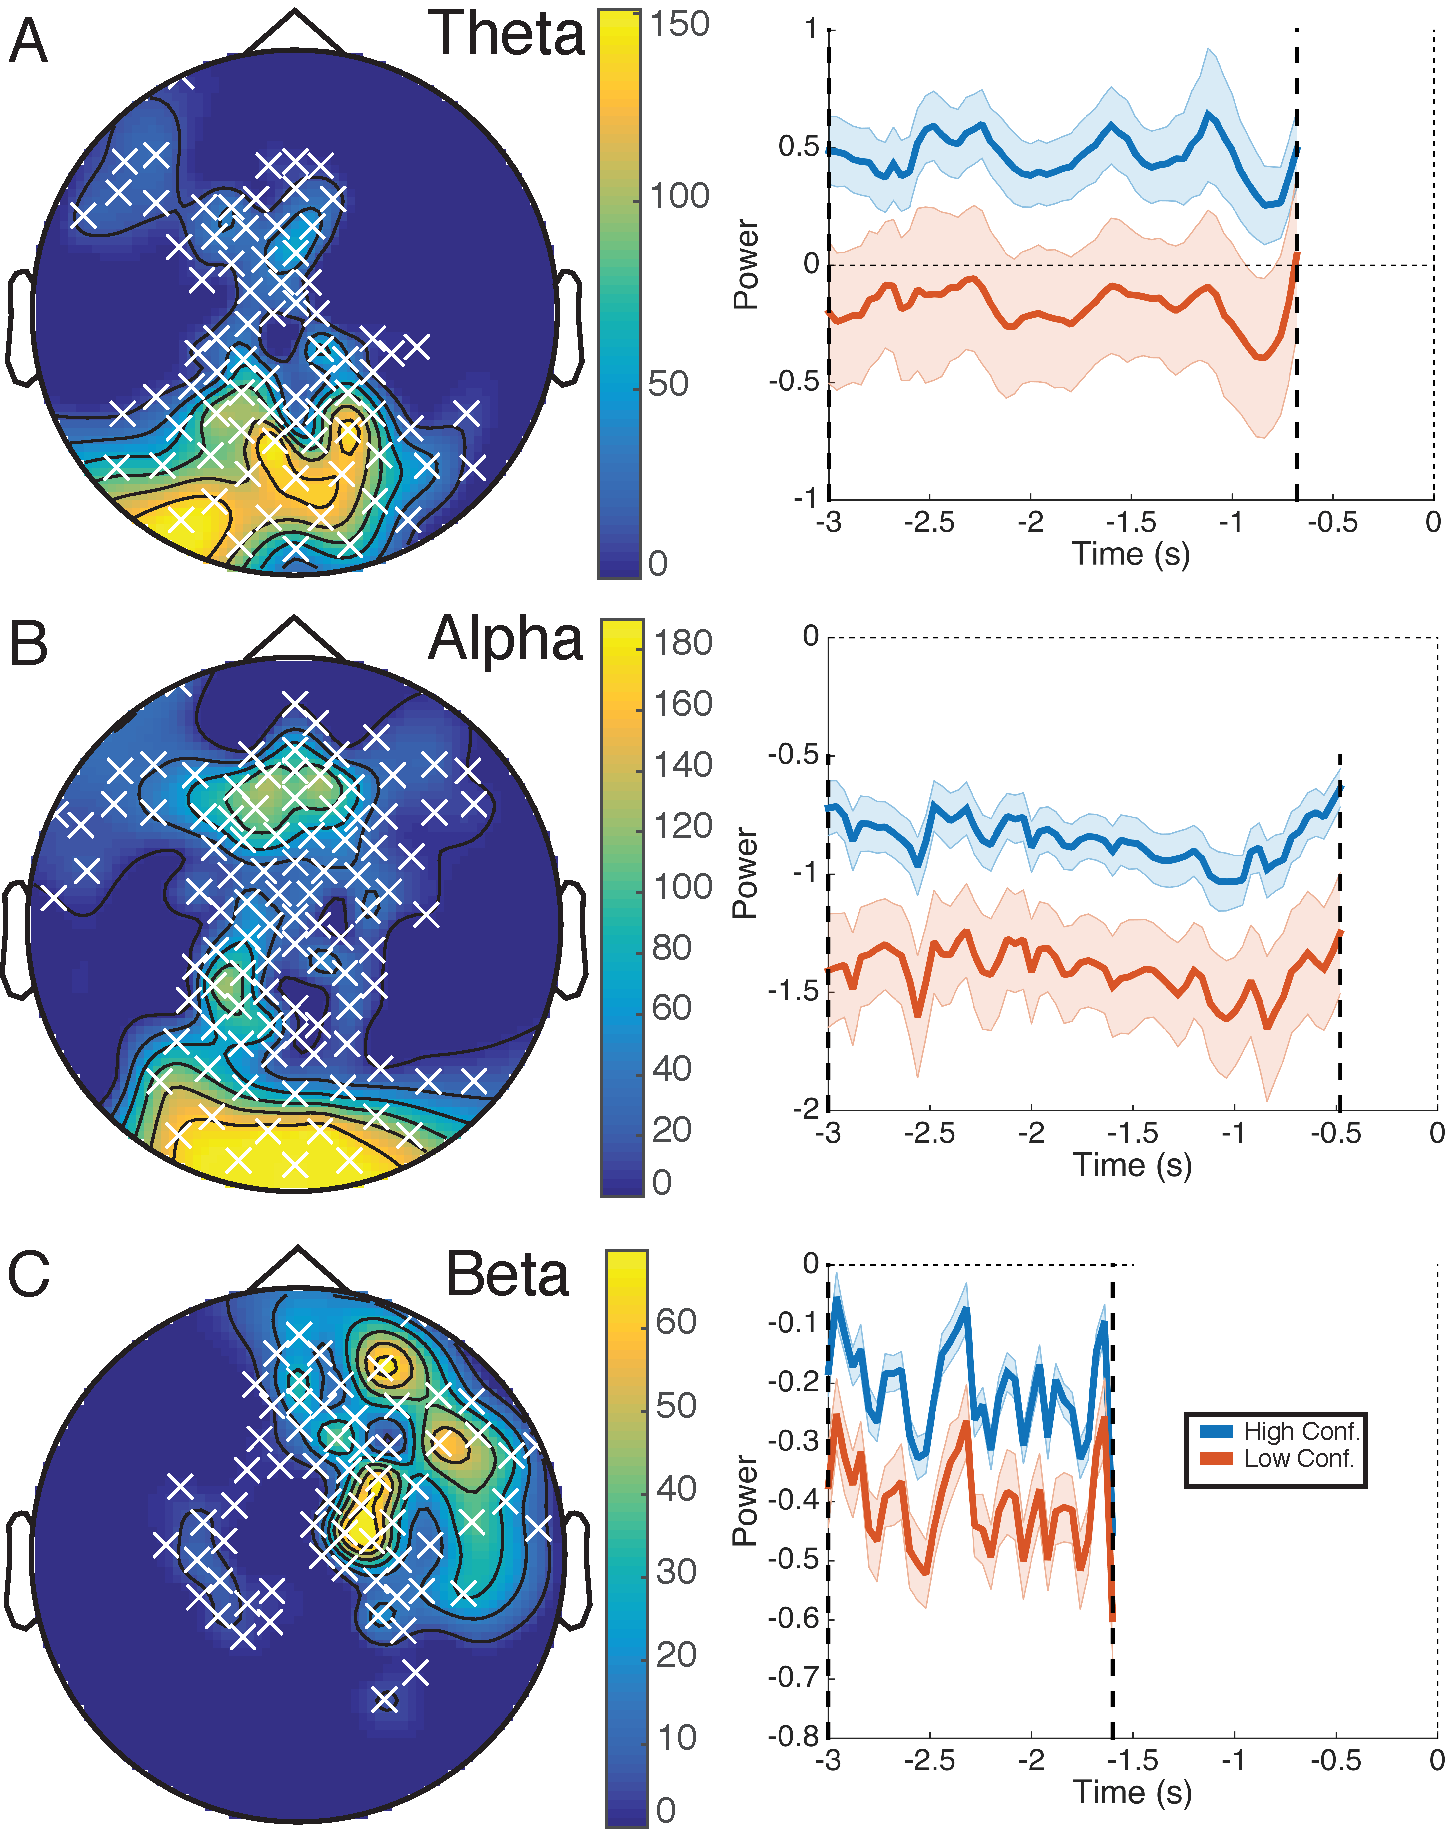
\includegraphics[width=.9\textwidth]{figs/deevConfClusters.pdf}
	\end{center}
	\caption[High vs. Low Confidence EEG Clusters]{
		\emph{(A)} Clustered found for response locked power difference between High vs. Low Confidence correct retrieval trials in the theta band.  On the left is the summed $t$-values over time for significant electrodes, on the right is the average power across significant electrodes for High Confidence shown in blue and Low Confidence shown in red.  Large dashed lines show the boundaries of the significant temporal window.
		\emph{(B)} Alpha cluster found for same contrast  as in A, here Low confidence trials show a greater decrease from baselined compared to high confidence trials.
		\emph{(C)} Beta cluster found, with similar properties to the alpha cluster in B.  
	}
	\label{fig:deevConfClusters}
\end{figure}




\subsection{Theta-Phase Model}
\label{sec:HippModelValidation}

%add LEABRA details here?

Input patterns were constructed, and memory retrieval performance measured, based on the slot topology in the EC layers (as highlighted in Figure~\ref{fig:depNet}).  This slot structure is intended to capture the modality segregation within EC, and within each slot we assume there is a {\em vocabulary} of different patterns, which reflect the representational repertoire within those modalities.  These vocabulary patterns were similarly used to estimate error within the networks' output by comparing, within a given slot, the output pattern of activation with all other vocabulary patterns.  If, for the given input pattern, the slots' output at the $\mathrm{EC}_{out}$ layer is closest to the vocabulary pattern it was trained on, it is considered correct, and otherwise considered incorrect.  This closest-pattern calculation is done across each of the slots for every input pattern, and if any slot shows an incorrect response the network output for that input pattern is counted as incorrect.  This measurement is referred to as \emph{Name Error} in the results section, and is thought to better represent the potential for clean up of hippocampal output as compared to more standard measures such as Sum Squared Error (SSE).    It also has the advantage of not requiring any further threshold or other parameterization.  It should be noted that this measure of error, compared to a SSE, deemphasizes single unit based errors in output in favor of an emphasis on distributed patterns of error across groups of units.


\section{Attentional Modulation: Deep LEABRA}
\label{appDeepLeabra}

The `Deep LEABRA' framework currently being developed in the Emergent software is the initial explorations into the modeling of interactions between thalamic relay nuclei, and superficial vs. deep cortical layers \cite{OReillyWyatteRohrlich14}.  This framework proposes that the neocortex is composed of two separable networks: superficial and deep/thalamic. The superficial-layer network consists of neocortical layers 4, 2, and 3, across different brain areas.  The deep/thalamic network starts in each cortical area with the layer 5b intrinsic bursting (IB) neurons, which receive inputs from local superficial neurons and top-down projections from other areas, and provide strong driving feedforward input to higher-order thalamic nuclei. These 5IB neurons also project to deep layer 6 cortical-thalmic (6CT) neurons, which interconnects with the thalamus (which in turn projects back up to layer 4 of the superficial network and layer 6 in the deep network).  This connectivity is illustrated in Figure \ref{fig:attn_compute}.  The current work takes advantage of the biological referents and computational implementation of the Deep LEABRA frameworkm however, here it is used as a simple form of attentional modulation (and not a temporal learning mechanism as described in \textcite{OReillyWyatteRohrlich14}).  The minimal description of the components necessary for this implementation are described below.  

The modulation of standard LEABRA unit activations (referred to as superficial units here) based the Deep LEABRA framework and the thalamic gating model described in \textcite{KetzJensenOReilly15} is carried out in two basic steps.  First, a Thalamic Relay Cell (TRC) unit receives input based on the threshold filtered output of some upstream units which have received its input from processing a given stimulus (in this case the hippocampus is providing this top-down modulation based on what is being retrieved).  These sending units, for a given TRC, are assumed to be the cortical thalamic projections from neocortical layers 5IB, 6CT \cite{ShermanGuillery06}, which reflect a thresholded filtering of superficial layer activity from both top-down and bottom-up sources. TRC activation dynamics are calculated in a similar manner to all LEABRA units, described in detail in \cite{KetzMorkondaOReilly13}, with the exception that its inputs are subject to an activation threshold of 0.1, and the weighted connections into and out of the TRC are not learned but instead remain fixed at 0.8.  

Second, the TRC activation is used to calculate the attentional modulation that it sends to down stream superficial units.  The attentional modulation is implemented through a separate set of activations for receiving units that can be considered an attentional mask that gets applied.  This mask is the TRC activation normalized to a range between some pre-determined minimum and a maximum of 1.  The effective modulation of the receiving unit is simply the multiplication of this attentional mask, and the receiving units' net input.  Thus, where activations are strong in the mask, the corresponding superficial layer activations will remain strong, but where they are weaker, the superficial layer activations will be reduced.  This modulation process is hypothesized to be carried out by layer 6CT neurons  \cite{BortoneOlsenScanziani14,OlsenBortoneAdesnikEtAl12}.

This multiplicitive modulation is based off previous mathematical models of attention that capture many of the effects relevant to the perception literature \cite{ReynoldsHeeger09,MontijnKlinkVanWezel12}.  Figure \ref{fig:attn_compute} shows how this framework captures the essential computations of the \textcite{ReynoldsHeeger09} model in different parts of the superficial and deep layer circuits.  Computationally, the TRC activations encode the attentional modulations of the superficial layer state. The attentional modulation signals cause the iterative constraint satisfaction process in the superficial network to focus on task-relevant information while down-regulating responses to irrelevant information, consistent with the abstract \textcite{ReynoldsHeeger09} mode.  Its important to note that this process can work in both a top-down (shown in \ref{fig:attn_compute}) and bottom-up fashion. Biologically, the layer 6CT neurons are known to exhibit a multiplicative influence over firing of superficial-layer neurons, in a manner consistent with the \textcite{ReynoldsHeeger09} model \cite{BortoneOlsenScanziani14,OlsenBortoneAdesnikEtAl12}. 


\begin{figure}
  \centering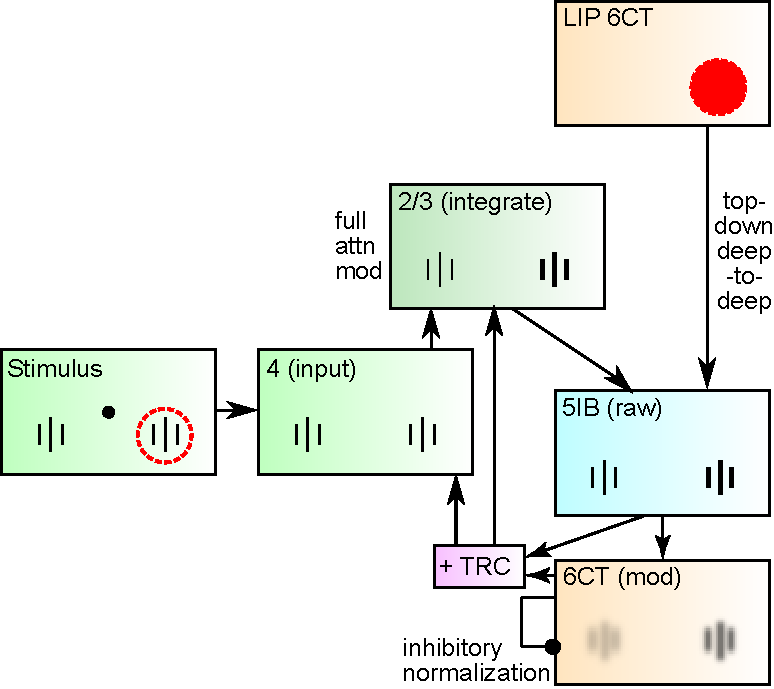
\includegraphics[width=.75\textwidth]{figs/fig_deepleabra_attn_compute.pdf}
  \caption[Signal Flow Through Cortical Layers in Deep LEABRA]{\small How attentional modulation is computed in response to a top-down attentional focus.  Layer 4 receives bottom-up sensory input, which then drives superficial layers (2/3), which initially do not reflect the attentional modulation (not shown).  The deep layer 5 Intrinsic Bursting (5IB) neurons integrate deep-to-deep top-down attentional inputs plus the local stimulus features from 2/3, to produce a {\em raw} deep output, prior to the contextual normalization process.  Layer 6 Cortical-Thalamic (6CT) neurons then integrate this direct activation from 5IB, to produce, for the first time in the circuit, a properly renormalized multiplicative gain-field activation pattern, with surround inhibition both within the 6CT layer and further downstream in the  TRC circuit providing the renormalization process.  These 6CT activations then modulate (multiply) the superficial-layer activations to produce {\em both} an increase in the attended location, and a decrease for the unattended location, as shown.  
  %In biological systems, this modulation also affects the layer 4 inputs (not shown) as well as 2/3, however, our model subsumes layer 4 into layer 2/3 neurons.
  }
  \label{fig:attn_compute}
\end{figure}

\subsection{Dependent Events Example Stimuli}
\label{appStimuli}

Below is an example set of events generated for the Dependent Events paradigm.  These stimuli were originally adapted from \textcite{HornerBisbyBushEtAl15}, where some original elements were removed due to British vs. American ubiquity, and replace with more common American elements.  The first 18 events are open loop, and the last 18 are closed loop with the appropriate balancing of object and animal stimuli.  


\begin{longtable}{l|c|c|c|c} \small
	\bfseries Event Number & \bfseries Location & \bfseries People & \bfseries Objects & \bfseries Animals  % specify table head 
	\csvreader[head to column names]{evts.csv}{}% use head of csv as column names
	{\\\hline\EventNumber & \Locations & \People & \Objects& \Animals}% specify your coloumns here
\end{longtable}



\printbibliography

\end{document}